\section{Background}
% Summarize the themes/aspects from the lecture course which are relevant for the paper which you will discuss. 
% 
In this part the basics are discussed. In order to understand the recent developments in LET technology, first the field effect, and transistor and LED technology must be understood. A short introduction to LETs is also given, and brief consideration to why development of organic semiconductors is important.
 
\subsection{Transistors}

The ability to on a large scale produce transistors has been one of the biggest advancements in the 20th century. Transistors and derived devices are necessary components in every modern electronic device. They can amplify currents or switch them off completely. To make these transistors, one needs a material that is capable of showing both characteristics of metals and of insulators, to be able to not only conduct currents, but also switch them off. These materials are called semiconductors, which have a band gap between the valence band and the conduction band. A pure semiconductor material behaves as an insulator, therefore doping of the material is needed to give it the metal-like properties.

\begin{figure}[!ht]
 \begin{center}
  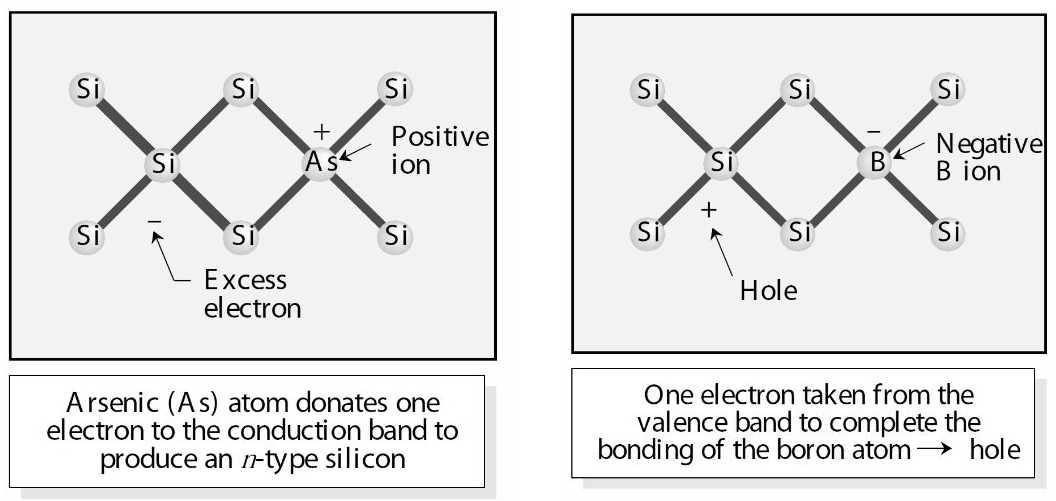
\includegraphics[width=1\textwidth]{doping}
  \caption{$n$-type doping and $p$-type doping. From \citet{vanweesbook}.}
  \label{fig:doping}
 \end{center}
\end{figure}

Doping (figure \ref{fig:doping}) introduces either extra electrons ($n$-type doping) or extra holes ($p$-type doping) in a material. This is done by putting atoms with different covalent bond forming properties in the crystals. With silicon, which forms 4 covalent bonds, to introduce extra electrons a material which forms 5 covalent bonds (e.g. arsenic) should be used. The extra electron is now relatively free to move. For p-type doping a material that only forms 3 covalent bonds (e.g. boron) should be used. The `empty' place is a hole which can travel relatively easy through the material.

Field-effect transistors are made of a combination of $n$-type and $p$-type semiconductors. The field effect refers to the control of the electrical conductivity of a material by the application of an external electric field. The working of a junction-FET (JFET) illustrates how this field effect is used. There are other transistor designs that use the field effect in a similar way, a few of which are the MOSFET, MESFET, and the organic OFET.

\begin{figure}[!ht]
 \begin{center}
  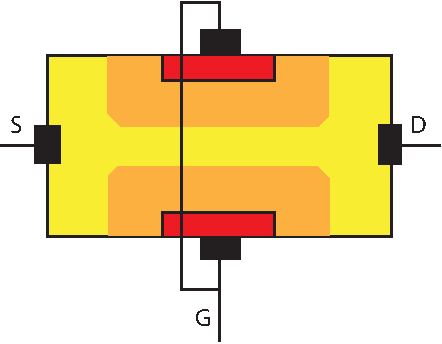
\includegraphics[width=0.7\textwidth]{jfet}
  \caption{A junction field effect transistor, with the position of source (S), drain (D) and gate (G) shown. Red is the substrate, yellow is the channel. Orange is the depletion zone influenced by the gate voltage.}
  \label{fig:JFET}
 \end{center}
\end{figure}

In figure \ref{fig:JFET} a diagram of a JFET is shown. In this example the channel through which the charge carriers flow (with a voltage difference between source and drain), is made of a $p$-type semiconductor, and the surrounding substrate is made of an $n$-type semiconductor. Therefore the mobile charge carriers in the channel are holes. When the mobile electrons in the substrate are pulled away by a positive voltage applied to the gate, only the static positive charges remain, which forms the depletion zone. This induces a positively charged electric field, which penetrates into the channel and repels the holes there, effectively narrowing the channel. With a high enough gate voltage the channel can be completely `pinched off', resulting in a voltage-controlled switch.

\subsection{Diodes}
Not only the transistor has had a big impact on society, the field of light-emitting materials has also seen much progress. From indicator lamps to replacements for incandescent light bulbs, the light-emitting diode (LED) has gained a lot of ground.

\begin{figure}[!ht]
 \begin{center}
  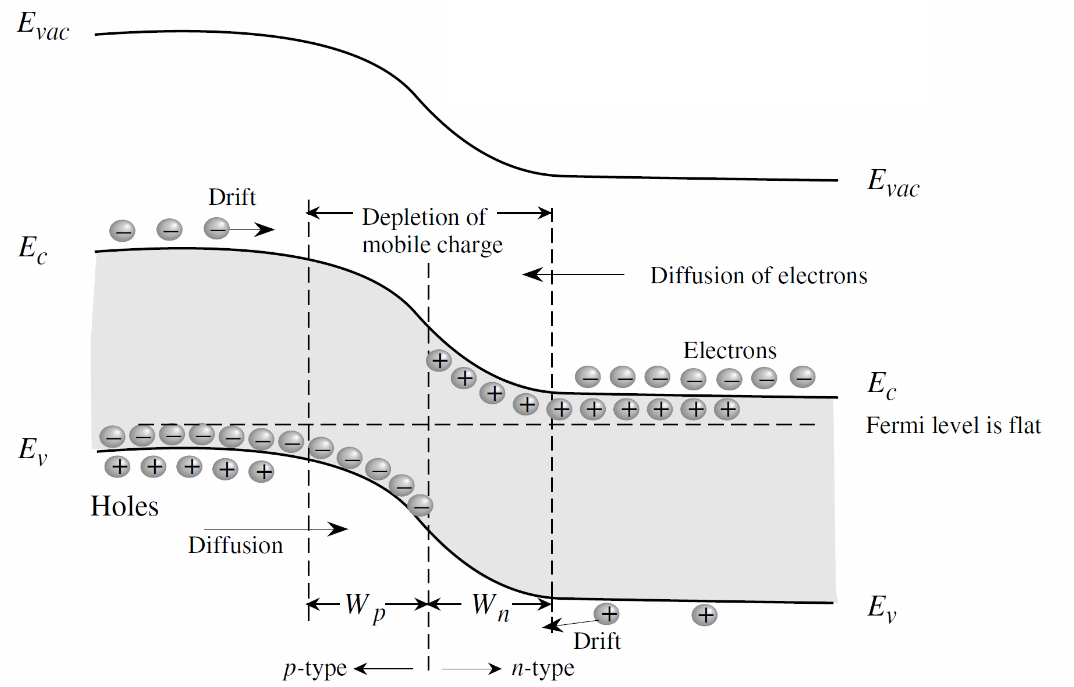
\includegraphics[width=0.8\textwidth]{pn_junction}
  \caption{$p$-$n$ junction. From \citet{vanweesbook}.}
  \label{fig:pn_junction}
 \end{center}
\end{figure}

To make an LED, one needs a $p$-$n$ junction. This is a piece of $p$-type semiconductor and $n$-type semiconductor put together. There is a difference in electron and hole densities across the junction, which results in the diffusion of holes from the $p$-side and electrons from the $n$-side. These recombine and near the junction only the static charges remain, which is called the depletion zone. In this region an electric field exists that repels the electrons and holes that enter the region.

If the $p$-type is connected to the positive terminal of a battery, and the $n$-type to the negative terminal (called forward bias), holes from the $p$-side and electrons from the $n$-side are pushed to the depletion zone. The width of the zone is reduced and with enough voltage difference the electrons and holes can go through the depletion zone and recombine with the charge carriers on the other side. Photons with the energy of the band gap of the materials are emitted. This is called electroluminescense and is the basis for an LED.

\subsection{LETs}

A light-emitting field-effect transistor (LET) is a device that couples the electrical characteristics of a FET to the controlled radiative recombination of the electrons and holes, which are injected into the channel via the source and drain contacts \citep{Muccini}. As seen in figure \ref{fig:LET}, the LET also has characteristics similar to a LED. Important is that the materials are able to sustain both electron and hole currents and efficient electroluminescense emission, to get a high quantum efficiency.

\begin{figure}[!ht]
 \begin{center}
  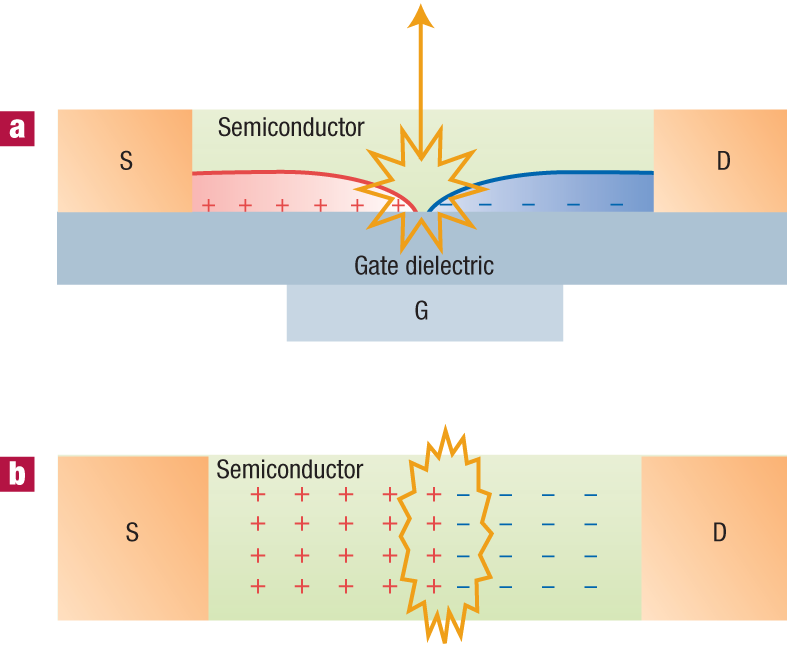
\includegraphics[width=0.6\textwidth]{fig_B1}
  \caption{Scheme of LET. (a) Side view. (b) Top view. The device can be thought of as a sort of forward-biased $p$-$n$ junction. Electrons and holes are injected from the drain (D) and source (S) contacts and recombine within the channel in a position controlled by the gate (G). From \citet{Muccini}.}
  \label{fig:LET}
 \end{center}
\end{figure}


\subsection{Organic Semiconductors}
In the previous sections the general structure of different devices were discussed, but not much was said about the materials that can be used to make these devices. Only silicon was talked about, however, there are many other suitable materials. A considerable amount of time and effort has been put into the development of organic semiconductors, and not without success. They are made from polymers, a base building block repeated many times. Often these building blocks are variations on the benzene ring. Organic semiconductors have many advantages over inorganic semiconductors, as summarized in the opto-electronics part of the course \citep{loinotes}. Unfortunately organic semiconductors also have disadvantages, which are surmountable depending on the purpose of the devices.

\begin{figure}[!ht]
 \begin{center}
  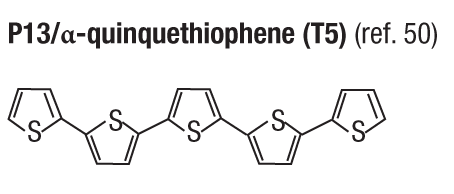
\includegraphics[width=0.4\textwidth]{zwavelbenzeen}
  \caption{Example of polymeric material. From \citet{Muccini}.}
  \label{fig:zwavelbenzeen}
 \end{center}
\end{figure}

Inorganic semiconductors require an expensive and complicated production method which involves several steps, including photo-lithography, etching, and metallization. Organic semiconductors on the other hand can be easily printed from a solution, and on many different types of (cheaper) materials such as glass, metal foils, and plastics, which as a bonus gives the possibility of producing flexible semiconductors. The organic semiconductor material itself is also much cheaper and more widely available.

With bulk inorganic semiconductor material it is not possible to change the bandgap considerably, which for LEDs restricts the wavelength of the light that comes out. One way to overcome this is by making nanocrystals: the size controls the wavelength. For organic semiconductors however it is much easier to change the bandgap. Most of the organic materials have a relative complex molecular structure compared to inorganic materials, and therefore there are more possibilities to adjust the molecule slightly resulting in different properties.

Against the major advantages that organic semiconductors have, there are a few disadvantages as well. For OLEDs the carrier mobility is about five orders of magnitude lower than of inorganic LEDs \citep{Muccini}. Even though the mobility for OLETs can be four orders of magnitude higher than OLEDs, it is still lower than that of inorganic materials. This means that the device reacts more slowly, which is not preferable.

Although the efficiency of organic devices continues to increase, for high brightness it still is not at the level of inorganic devices. The efficiency is described by the quantum efficiency $\eta$: the fraction of excited carriers that recombine radiatively. The corresponding equation is:
\[
 \eta = \frac{R_{r}}{R} = \frac{\tau_{nr}}{(\tau_{tr}+\tau_{nr})},
\]
with $R=$ total recombination rate, $R_{r}=$ radiative recombination rate, $\tau_{tr}=$ radiative lifetime, and $\tau_{nr}=$ non-radiative lifetime. The goal is to have an as high as possible radiative recombination rate, because only those recombinations emit light.

Finally the lower lifetime of organic semiconductors is worth some consideration. Their lifetime is lower compared to inorganic semiconductors, and they are more vulnerable to the environment. This is because organic materials react more easily with water or oxygen. 
